\documentclass[10pt,a4paper]{article}
\usepackage[utf8]{inputenc}
\usepackage[catalan]{babel}
\usepackage{amsmath}
\usepackage{amsfonts}
\usepackage{amssymb}
\usepackage{graphicx}
\usepackage[left=2cm,right=2cm,top=2cm,bottom=2cm]{geometry}
\usepackage{hyperref}
\hypersetup{
    colorlinks=true,
    linkcolor=cyan,
    anchorcolor=cyan,
    filecolor=cyan,      
    urlcolor=blue,
}

\usepackage{fancyhdr}
\pagestyle{fancy}
\usepackage{xcolor}
\usepackage{titling}

\usepackage{listings}
\usepackage{color}

%New colors defined below
\definecolor{codegreen}{rgb}{0,0.6,0}
\definecolor{codegray}{rgb}{0.5,0.5,0.5}
\definecolor{codepurple}{rgb}{0.58,0,0.82}
\definecolor{backcolour}{rgb}{0.95,0.95,0.92}

%Code listing style named "mystyle"
\lstdefinestyle{mystyle}{
  backgroundcolor=\color{backcolour},   commentstyle=\color{codegreen},
  keywordstyle=\color{magenta},
  numberstyle=\color{codegray},
  stringstyle=\color{codepurple},
  basicstyle=\scriptsize\ttfamily\tiny,
  breakatwhitespace=false,         
  breaklines=true,                 
  captionpos=b,                    
  keepspaces=true,                                     
  numbersep=5pt,                  
  showspaces=false,                
  showstringspaces=false,
  showtabs=false,                  
  tabsize=2,
  framextopmargin=1pt,
  framexbottommargin=10pt,
}

\usepackage{sectsty}
\partfont{\large}

%"mystyle" code listing set
\lstset{style=mystyle}

%For generate trees
\usepackage{tikz}

% To generate a box with text and background
\definecolor{shadecolor}{RGB}{200,201,190}
\newcommand{\mybox}[1]{\par\noindent\colorbox{shadecolor}
{\parbox{\dimexpr\textwidth-2\fboxsep\relax}{#1}}}

% change part number to arabic
\renewcommand{\thepart}{\arabic{part}}

\author{Ruben Vasallo Gonzalez}
\title{Tipologia i cicle de vida de les dades \\ PRAC 1 \\ 2018-2019}

\headsep = 1,5cm
\lhead{\begin{picture}(0,0) \put(0,0){
\includegraphics[width=2cm]{logo-uoc-default.png}} \end{picture}}
\chead{}
\rhead{\thetitle \\ \theauthor}


\begin{document}
\maketitle

\part*{Exercici d'extracció dels preus dels carburants del Principat d'Andorra.}

\section{Nom del dataset: Preu dels carburants al Principat d'Andorra.}

\section{Descripció}
Dataset on es mostren els preus dels diferents carburants a les gasolineres del Principat d'Andorra.

\section{Imatge}
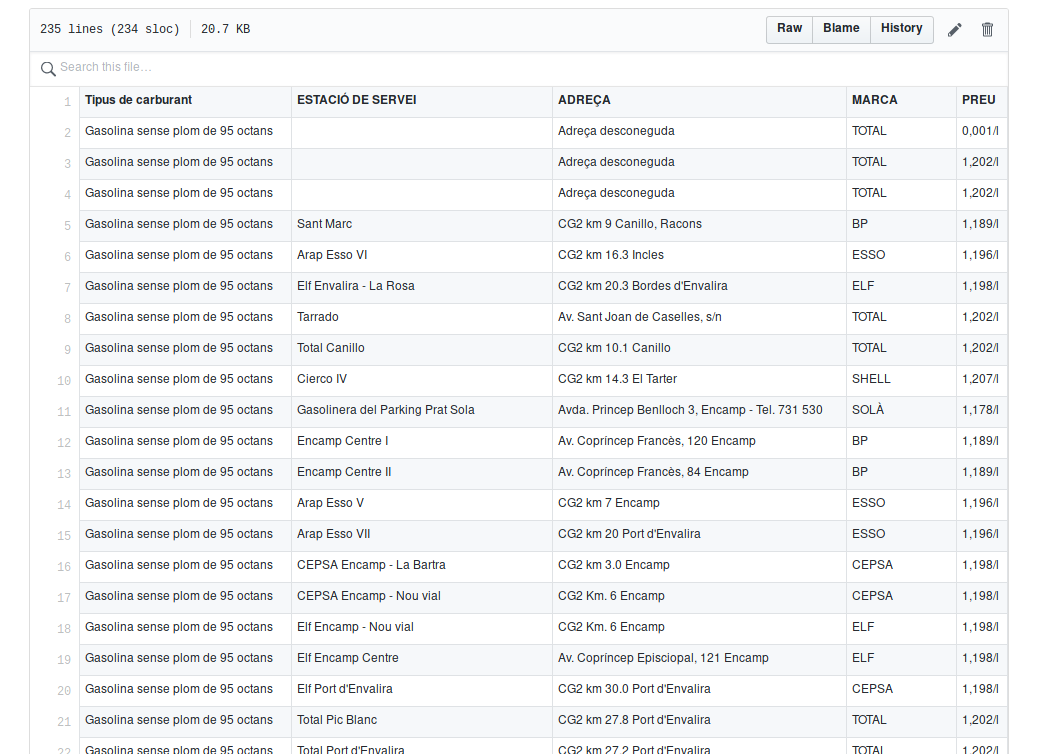
\includegraphics[width=16cm]{datset-image.png}

\section{Context}
El context d'aquest dataset es avaluar els preus que tenen els carburants en el Principat d'Andorra per a que els usuaris pugin valorar on es el millor lloc i/o dia per omplir els dipòsits dels seus vehicles. A mes a mes també disposem del preu del gasoil de calefacció que permetrà als usuaris escollir quin es el millor moment de l'any per omplir els dipòsits de casa seva.

\section{Contingut}
El dataset compren varis fitxers en format csv amb la mateixa estructura per cadascun d'ells. Com la informació d'origen s'ofereix només diàriament, el període d'aquest dataset es el de varies dies separant per fitxers classificats per el dia que es va recollir la informació. A continuació indiquem el camps que tenen el dataset:

\paragraph*{}
\textbf{- Tipus de carburant:} Tipus del carburant al que fa referencia l'observació.

Pot tenir els següents valors: \textit{[Gasolina sense plom de 95 octans, Gasolina sense plom de 98 octans, Gasoil de locomoció, Nou gasoil de locomoció i Gasoil de calefacció]}

\textbf{- Estació de servei:} Nom de l'estació de servei al que fa referencia l'observació.

\textbf{- Adreça:} Adreça de l'estació de servei al que fa referencia l'observació.

\textbf{- Marca:} Marca de l'estació de servei al que fa referencia l'observació.

\textbf{- Preu}: Preu en euros per litre del carburant al que fa referencia l'observació.

\section{Agraïments}
Agraïm al ministeri de Medi Ambient i Sostenibilitat del Govern d'Andorra per facilitat a traves de la seva web les dades necessaris per crear aquest dataset.
\paragraph*{}
Podeu consultar més dades a la seva web: \href{https://www.mediambient.ad/energia/preus-dels-carburants}{https://www.mediambient.ad/energia/preus-dels-carburants}

\section{Inspiració}
La crisis a afectat a totes les economies del mon, i no es cap bogeria dir que avui dia, es te que mirar mes que mai els gast que una família a de fer front. A mes a mes, si afegim a la ja difícil situació, que vius en un àrea on la mobilitat amb vehicle privat o la calefacció de la teva llar es necessari (per no dir imprescindible) per a poder viure, amb mes motiu es te que mirar el consum per poder fer front al gast a final de mes. Com hem comentat anteriorment, l'idea es la de tenir tota la informació necessària per poder decidir amb coneixement quin i quan es el millor moment per poder omplir de carburant els nostres vehicles o el diposit de la calefacció de la teva casa. Inclús amb un dataset prou ampli es podrien fer entrenament de models predictius per intentar prediu re les tendències dels preus d'aquests.

\section{Llicència}

Després d'analitzar les possibles llicencies que existeixen, he escollit publicar tant el codi com el resultat d'aquest (el dataset resultant) amb la llicencia \textit{\href{https://creativecommons.org/licenses/by-nc-nd/4.0/deed.es}{CC BY-NC-ND (Attribution-NonCommercial-NoDerivs)}} Atribución-NoComercial-SinDerivadas 4.0 Internacional.

\paragraph*{}
He escollit aquesta llicencia després de comprovar que la web origen de les dades te "\textit{copyright}" vigent, a mes a mes d'analitzar la \href{https://www.mediambient.ad/avis-legal}{política d'us} que te la web font i veure que, en aquesta, es destaca que \textit{"Només està autoritzat l'ús personal de les imatges i arxius que es poden descarregar de la web. El seu ús comercial no està permès."}

\paragraph*{}
Considero que la llicencia \textit{CC BY-NC-ND} cobreix que nomes es pugin utilitzar les dades en el mateix sentit que en la web original, ja que aquesta llicencia no permet l'us de les dades amb intenció comercial de cap de les maneres.

\section*{Bibliografia}
\begin{itemize} \label{bibliography:1}
\item Tipus de llicencies Creative Commons $\Rightarrow$ \href{https://creativecommons.org/licenses/}{https://creativecommons.org/licenses/}
\item Pregues frequents sobre les lliciencies Creative Commons $\Rightarrow$ \href{https://creativecommons.org/faq/}{https://creativecommons.org/faq/}
\item Drets d'autor "\textit{copyright}" $\Rightarrow$ \href{https://es.wikipedia.org/wiki/Derecho_de_autor}{https://es.wikipedia.org/wiki/Derecho\_de\_autor}
\item Drets d'autor aplicats a Andorra $\Rightarrow$ \href{http://www.wipo.int/wipolex/en/text.jsp?file_id=187689}{http://www.wipo.int/wipolex/en/text.jsp?file\_id=187689}
\end{itemize}

\end{document}